

%-----------------------------------------------------------------------------%
\chapter{\babSatu}

%-----------------------------------------------------------------------------%
%-----------------------------------------------------------------------------%


\section{Latar Belakang}

%-----------------------------------------------------------------------------%
Bahasa merupakan representasi perilaku kompleks yang dimiliki oleh spesies dengan tingkat kognisi tinggi. Elemen suara, kata-kata, dan pola sintaktis sebuah bahasa berbeda untuk setiap kelompok manusia dan berkembang secara perlahan menjadi bentuk bahasa yang paling efisien \citep{aitchison2004change}. Hal ini disebabkan oleh berkembangnya pola linguistik seiring waktu dan penyebaran \citep{sapir1921intro}. \cite{chomsky1965syntactic} juga mengungkapkan bahwa keserupaan dari semua bahasa di dunia adalah aspek kreatifnya, sehingga memungkinkan penutur untuk mengekspresikan pikiran dengan jumlah yang tak terhingga dan bereaksi secara tepat dalam segala bentuk situasi. Salah satu karakteristik ujaran manusia yang paling utama adalah tingkat keteraturan atau organisasi isi tuturan yang sangat tinggi. Semua satuan yang membentuk sebuah tuturan disusun oleh penutur dengan konfigurasi yang sangat spesifik mengikuti aturan tertentu. Aturan-aturan ini membentuk tataran organisasi terpenting dari sebuah bahasa, yaitu sintaksis. Para linguis Jerman terdahulu menerjemahkan kata sintaksis ke dalam bahasa Jerman sebagai \textit{Satzlehre} atau 'ilmu kalimat' karena obyek dari sintaksis struktural adalah studi tentang kalimat \citep{tesniere1959elements}.

Dalam kajian-kajian linguistik transformasional, para linguis memisahkan antara pengetahuan penutur terhadap sebuah bahasa untuk dapat memproduksi dan memahami bahasanya dengan bagaimana penutur menggunakan pengetahuan tersebut secara nyata untuk berbicara, memahami, membaca, dan menulis (\citealp{chomsky1965syntactic,delahuntygarvey2010soundsense}). Manusia memiliki kemampuan mental dan kognisi untuk mempelajari, memproduksi, dan mengerti ujaran yang berbeda-beda. Pengetahuan bawah sadar terhadap aturan yang membentuk sebuah bahasa ini disebut dengan kemampuan (\textit{competence}). Sementara itu, aktivitas linguistik yang memanfaatkan pengetahuan tersebut secara nyata disebut dengan penampilan (\textit{performance}). \cite{chomsky1965syntactic} menekankan bahwa investigasi terhadap penampilan bahasa hanya akan bermakna sejauh pemahaman terhadap kemampuan bahasa yang mendasarinya.

Beberapa linguis lain seperti \cite{sagwasow2011pccg} berargumen dan mengungkapkan pentingnya penelitian mengenai penampilan bahasa yang dapat menjadi basis fakta empiris dalam perkembangan teori-teori gramatikal atau kemampuan bahasa. \cite{hawkins2014cross} juga mengeksplorasi keterkaitan antara penampilan bahasa dan konvensi tata bahasa dan mengungkapkan bahwa kecenderungan yang ditemukan dalam data penggunaan bahasa yang mencakup pilihan penutur (urutan kata, pilihan klausa, dan lain-lain) tampak serupa dengan kecenderungan yang ditemukan dalam konvensi tata bahasa. Hawkins berasumsi bahwa aturan tata bahasa sudah merefleksikan keterbatasan memori serta bentuk efisiensi dan kompleksitas lain yang diobservasi dalam data penggunaan bahasa atau penampilan bahasa. Namun, asumsi ini baru memiliki bukti kuat dalam penelitian terhadap bahasa-bahasa dengan urutan kata yang lebih pasti (\textit{fixed word order}). 

Berbagai penelitian lintas bahasa telah dilakukan untuk menunjukkan bahwa banyak bahasa di dunia tidak terkekang oleh struktur urutan kata sesederhana Subyek, Predikat, dan Obyek seperti dalam Bahasa Inggris yang urutan Subyek dan Predikat-nya bisa berubah (\citealp{macwhinneybates1989cross, birnerward1998noncanonical, lambrecht2000info}). Perbedaan urutan kata dapat dimotivasi oleh bebagai aspek seperti kala waktu, kepastian, dan \textit{animacy} (\citealp{dryer1992greenbergian, tsunoda1995adpositions, polinskaja1989object}).  \cite{hawkins1994performance} berargumen bahwa terdapat keterkaitan konsep urutan kata antara bahasa-bahasa dengan \textit{free word order} dan \textit{fixed word order}, yaitu bahwa urutan kata yang banyak digunakan oleh penutur pada bahasa dengan \textit{free word order} serupa dengan urutan kata yang dikonvensionalisasikan secara aktif pada bahasa dengan \textit{fixed word order}. \cite{hawkins1994performance} mengaitkan pilihan terhadap urutan kata tertentu ke dalam asas efisiensi bahasa yang dikembangkannya dan mengatakan bahwa jenis urutan kata tertentu memudahkan pendengar memproses informasi dibandingkan yang lain.

Kesimpulan bahwa bahasa Indonesia tergolong memiliki urutan kata yang bebas banyak muncul dalam penelitian mengenai urutan kata pada ranah sintaksis (\citealp{stack2005word, postman2004processing}). \cite{sneddon2010indonesian} mengungkapkan bahwa meskipun bahasa Indonesia memiliki basis urutan kata tertentu, berbagai kondisi memungkinkannya untuk berubah, seperti contoh perbedaan penekanan yang mengakibatkan perbedaan urutan kata antara "Endang lari ke toko dengan cepat" dan "Dengan cepat Endang lari ke toko". Dalam penelitiannya, \cite{postman2004processing} menekankan bahwa bahasa Indonesia merupakan bahasa yang berorientasi pada tema sehingga tidak memiliki urutan kata resmi yang jelas. Pada aspek efisiensi, John McWhorter menulis sebuah artikel di media online The Atlantic \citep{mcwhorter2016efficient} dengan memaparkan beberapa bukti ujaran dari penutur bahasa Indonesia untuk menunjukkan bagaimana bahasa Indonesia merupakan salah satu bahasa paling efisien dan ekonomis. McWhorter menambahkan bahwa tata bahasa dalam bahasa Indonesia juga secara periodik diolah secara organik oleh para penuturnya sehingga terdapat keteraturan bentuk bahkan dalam bahasa sehari-hari (informal). Urutan kata dan efisiensi dalam bahasa Indonesia ini sangat berkaitan dengan perdebatan antara hubungan kemampuan dan penampilan di dunia linguistik, terutama dikarenakan tingginya fleksibilitas yang dimiliki oleh bahasa Indonesia.

Selama puluhan tahun, banyak riset dilakukan untuk melihat bagaimana penutur mengatur dan memproduksi bahasa menjadi bentuk yang paling efisien (\citealp{chomsky2005three, hawkins2004efficiency, zipf1935psycho, zipf1949human}). Beberapa kajian linguistik modern yang menyoroti masalah ini memanfaatkan teori dependensi. Dependensi adalah gagasan bahwa setiap unit linguistik terhubung satu sama lain oleh tautan langsung karena memiliki relasi semantik \citep{tesniere1959elements}. Sebagai contoh, penutur bahasa Indonesia harus menuturkan Saya cinta kamu dan bukan *Saya kamu cinta seperti dalam bahasa Perancis (\textit{Je t'aime}). Pada kedua kalimat tersebut, terlihat perbedaan bagaimana posisi subyek dan obyek bergantung pada predikatnya. Contoh kasus sederhana tersebut menunjukkan bahwa kata-kata sebagai konstituen kalimat terhubung oleh tautan langsung yang disebut juga dengan dependensi (\textit{dependency}). Teori dependensi merupakan teori sintaksis modern namun memanfaatkan konsep dasar linguistik seperti halnya konsep penanda dan petanda yang digagas oleh Saussure \citep{key2017course}. 

Menurut Saussure, untuk dapat mengantarkan informasi tertentu, penutur harus memilih tanda pada sumbu paradigmatik dan mengatur tanda tersebut ke dalam urutan linear pada sumbu sintagmatik. Dalam teori dependensi, satu kata harus bergantung kepada kata lain untuk menduduki posisi linear tertentu dan membentuk relasi sintagmatik \citep{tesniere1959elements}. Dengan kata lain, pengaturan tanda pada sumbu sintagmatik dikendalikan oleh dependensi yang menghubungkan konstituen-konstituen tersebut. Perbedaan dependensi tidak hanya berlaku secara lintas bahasa seperti pada contoh kasus dalam bahasa Indonesia dan Perancis di atas, tetapi juga dapat ditemukan dalam satu bahasa seperti pada Gambar 1 sehingga dapat memberikan gambaran keterkaitan struktur konstruksi kalimat dengan kerja kognisi manusia \citep{gibson2000dependency}. Posisi kata keluar pada urutan linear kedua kalimat berbeda, sehingga jarak dependensi antara kata membuang dan keluar pada kedua kalimat juga berbeda (\pic~\ref{fig:contoh-dependensi}). 
\begin{figure}
	\centering 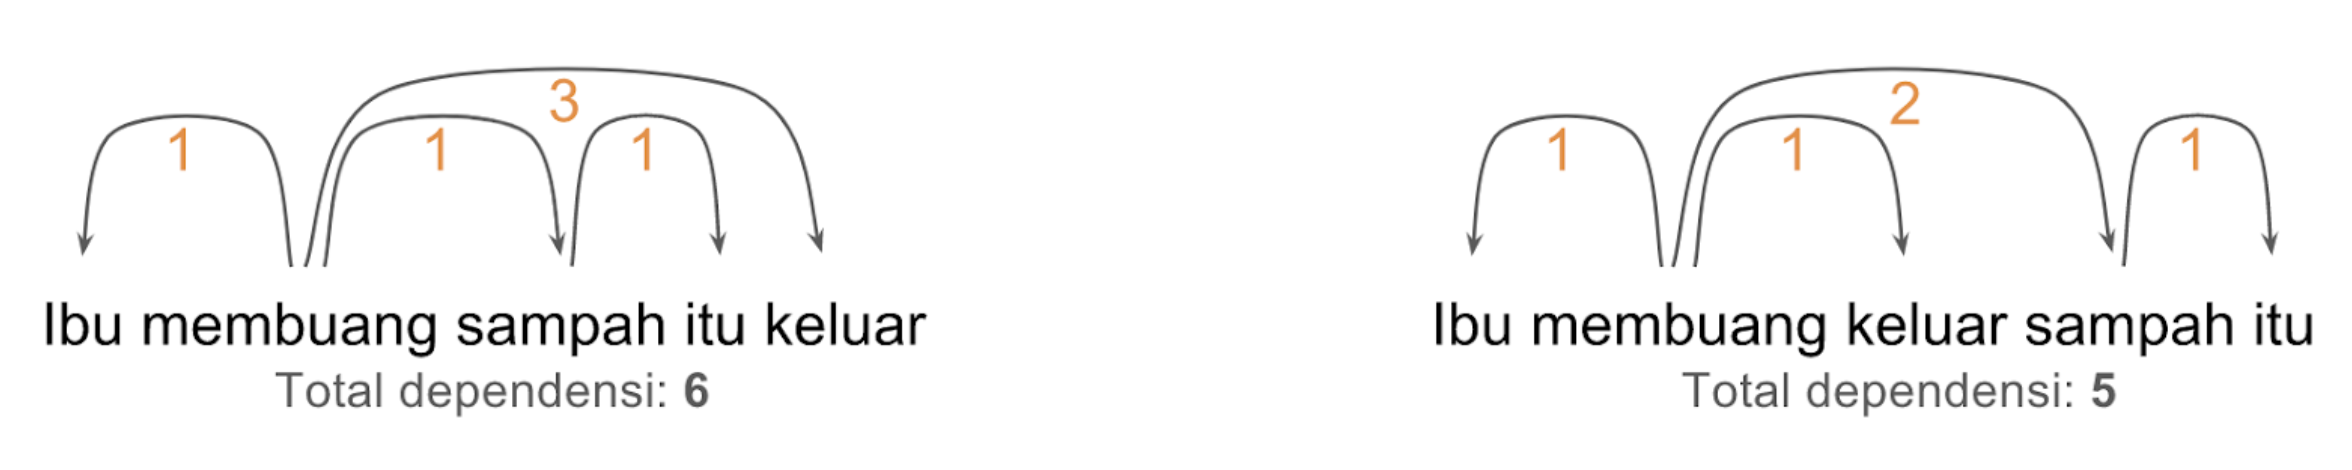
\includegraphics[width=1
	\textwidth] {pics/contoh-dependensi.png} \caption{Contoh perbedaan dependensi dalam bahasa Indonesia} 
\label{fig:contoh-dependensi} \end{figure}

Salah satu hipotesis yang membahas jarak dependensi menyebutkan adanya kecenderungan bahwa penutur akan mendekatkan kata-kata dalam kalimat yang memiliki relasi secara semantik \citep{futrell2015large}. Hipotesis ini sangat berkaitan dengan prinsip efisiensi yang dikembangkan oleh \cite{hawkins2004efficiency}. Kata-kata yang mendekat akibat pengurangan jarak dependensi ini juga dihubungkan dengan hipotesis adanya kesulitan dalam produksi dan pemahaman penutur terhadap ujaran dengan jarak dependensi yang jauh dan struktur yang rumit \citealp{hawkins2004efficiency, dillon2011structured}. Sebagai contoh, pada \pic~\ref{fig:contoh-dependensi}, kata membuang dan keluar memiliki tautan langsung sehingga memori kerja penutur akan bekerja untuk menghubungkan keduanya. Semakin jauh jarak keduanya, maka memori kerja akan bekerja semakin banyak. Konsep tersebut mendukung penelitian \cite{jaeger2006redundancy} yang mengungkapkan bahwa penutur cenderung untuk mengutamakan alasan efisiensi kerja memori tersebut dalam menyusun kata-kata dalam urutan linear pada sumbu sintagmatik, terutama pada ujaran yang lebih spontan \citep{jaeger2006redundancy}. \cite{futrell2015large} menemukan adanya fenomena pengurangan jarak dependensi antarkata dalam 37 bahasa yang termasuk di dalamnya adalah bahasa Indonesia. Dalam penelitian tersebut, \cite{futrell2015large} menyebutkan bahwa temuan dalam bahasa Indonesia menunjukkan tingkat pengurangan jarak yang paling tinggi dibandingkan 36 bahasa lainnya. 

Penelitian terdahulu dengan data bahasa Indonesia yang mengungkit dependensi (\citealp{kamayani2011dependency, green2012indonesian, irmawati2015dependency, futrell2015large}) memanfaatkan korpus bahasa Indonesia mencakup data ragam tulis dari media jurnalistik daring, blog, artikel penelitian, dan media sosial. Pemilahan data dalam penelitian-penelitian tersebut hanya didasarkan pada keragaman serta kuantitas data. Berdasarkan hasil temuan \cite{wang2017effects}, genre atau jenis teks hampir tidak berpengaruh terhadap pola distribusi jarak antarkata yang memiliki relasi semantik. Hal ini berarti terlepas dari jenis teks, manusia cenderung untuk meminimalisir jarak dependensi pada kondisi tertentu \citep{wang2017effects}. Di lain sisi, \citep{wang2017effects} menemukan bahwa teks imajinatif cenderung memiliki jarak dependensi yang lebih panjang dibandingkan dengan teks informatif sehingga teks informatif lebih mudah untuk dimengerti\footnote{Penelitian \cite{wang2017effects} memanfaatkan British National Corpus yang mencakup teks informatif seperti berita dan laporan serta teks imajinatif seperti literatur fiksi dan dialog film.}. Namun, \cite{miller2011critical} mengkaji adanya perbedaan kerumitan sintaktis dalam teks informatif itu sendiri, seperti halnya media cetak formal akan lebih kompleks dibandingkan dengan artikel tabloid. Hal ini menunjukkan bahwa data penelitian linguistik terkait dependensi dapat fokus kepada salah satu jenis teks (informatif atau imajinatif) dan tetap mendapatkan gambaran keragaman pola yang ada di dalamnya. Keterbatasan lain yang dihadapi apabila melibatkan data bahasa sehari-hari (non-formal) adalah kurangnya sumber daya teknologi untuk mengolah data tersebut \citep{green2012indonesian}. Dalam banyaknya pembahasan secara global mengenai efisiensi dipandang dari segi dependensi dalam linguistik, terdapat kerumpangan terkait ranah tersebut dalam bahasa Indonesia. Kajian-kajian terdahulu yang menyinggung teori dependensi untuk bahasa Indonesia dilakukan oleh para peneliti terbatas untuk mengembangkan perangkat atau metode komputasional untuk penguraian kalimat berdasarkan dependensinya (\citealp{kamayani2011dependency, green2012indonesian, irmawati2015dependency}). Hingga saat ini, belum ada kajian yang dapat memberikan wawasan dari aspek linguistik tentang bagaimana penutur menyusun struktur ujaran atau kalimat terkait pengurangan jarak dependensi dalam bahasa Indonesia. Terkait dengan kerumpangan tersebut, belum ada juga kajian yang memanfaatkan bukti penampilan produksi ujaran yang lebih spontan melalui data ragam lisan sebagai salah satu data utama penelitian. 

%-----------------------------------------------------------------------------%


\section{Perumusan Masalah}

%-----------------------------------------------------------------------------%
Urutan kata dalam kalimat pada bahasa Indonesia tidak terkekang aturan konstruksi dibandingkan dengan bahasa lain seperti Inggris dan Jerman (\citealp{stack2005word, futrell2015large, irmawati2015dependency}). \cite{kubler2009dependency} menyebutkan bahwa teori dependensi sangat sesuai untuk dimanfaatkan dalam menelaah bahasa dengan karakter urutan kata yang bebas (\textit{free word order}) seperti bahasa Indonesia. Tingginya tingkat pengurangan jarak dependensi antarkata yang ditemukan dalam bahasa Indonesia \citep{futrell2015large} juga menunjukkan adanya keragaman pola pengurangan jarak dependensi antarkata dalam bahasa Indonesia.

Terkait dengan latar belakang di atas, muncul satu pokok permasalahan yang diuraikan dalam penelitian ini yaitu \textbf{bagaimana penutur bahasa Indonesia menyusun stuktur ujaran yang efisien dipandang dari segi dependensi pada ragam tulis dan lisan}. Dengan memanfaatkan korpus data jurnalistik bahasa Indonesia termutakhir ragam tulis dan lisan yang terkumpul, pokok permasalahan ini diuraikan menjadi tiga pertanyaan yang lebih detail:

\begin{enumerate}
	\item Bagaimana pengaruh panjang kalimat dalam penyusunan struktur ujaran atau kalimat yang efisien dalam bahasa Indonesia dipandang dari segi dependensi?
	\item Bagaimana efisiensi ujaran tercermin pada jarak dan arah dependensi antarkonstituen dalam bahasa Indonesia?
	\item Bagaimana pengaruh penyusunan struktur ujaran yang efisien dalam bahasa Indonesia dipandang dari segi dependensi terhadap valensi akar?
\end{enumerate}

\section{Tujuan Penilitian}

%-----------------------------------------------------------------------------%
Penelitian ini memiliki tujuan utama untuk memaparkan strategi penutur bahasa Indonesia dalam menyusun struktur ujaran atau kalimat yang efisien dipandang dari segi dependensi yang dijabarkan melalui pengaruh panjang kalimat terhadap penyusunan ujaran, jarak dan arah dependensi antarkata, serta pengaruh urutan konstituen terhadap valensi konstituen induk. Beberapa aspek sintaksis terkait pembentukan struktur ujaran ini diuraikan untuk menguji hipotesis pengurangan panjang dan jarak dependensi antarkonstituen dalam sebuah ujaran seperti yang telah dibahas oleh beberapa penelitian terdahulu. Hasil penelitian ini berupa gambaran umum pengurangan panjang dan jarak dependensi pada beberapa aspek pembentukan struktur ujaran dan uraian secara mendalam mengenai tautan-tautan dependensi yang terjadi antara konstituen induk dan konstituen terikatnya. Penelitian ini menitikberatkan pada analisis penampilan linguistik dengan memanfaatkan data penggunaan bahasa Indonesia secara nyata sebagaimana tercermin dalam korpus jurnalistik bahasa Indonesia ragam tulis dan lisan.

%-----------------------------------------------------------------------------%


\section{Manfaat Penelitian}

%-----------------------------------------------------------------------------%
Jika penyusunan struktur ujaran yang digunakan penutur baik secara produksi maupun pemahaman didorong oleh motivasi untuk memudahkan kesulitan berkomunikasi, maka ekspektasi utama adalah penghindaran terhadap tautan dependensi yang jauh \citep{futrell2015large}. Hipotesis pengurangan panjang dan jarak dependensi ini dapat berperan sebagai kerangka untuk menjelaskan hubungan antara bagaimana penutur memanfaatkan dan menyusun struktur sintaksis sebuah bahasa dengan tujuan utama untuk menciptakan komunikasi yang efisien meskipun dengan ujaran yang bersifat kompleks.
%-----------------------------------------------------------------------------%

\subsection{Manfaat untuk pengembangan ilmu linguistik (teoretis)}
%-----------------------------------------------------------------------------%
Secara teoretis, penelitian ini dapat menjadi dasar pengembangan ilmu sintaksis modern yang kontekstual karena menitikberatkan pada penampilan linguistik yang dapat memberikan bukti-bukti kuat atas kemampuan linguistik. Bukti-bukti penampilan bahasa dalam penelitian ini juga dapat ditindaklanjuti untuk merumuskan pengajaran ilmu sintaksis yang responsif terhadap penggunaan bahasa yang nyata dalam masyarakat. Selain itu, penelitian ini dapat dimanfaatkan oleh bidang perencanaan bahasa untuk memaknai penggunaan bahasa dalam masyarakat berdasarkan urutan kata-kata (\textit{word order}) terkait dengan perkembangan relasi sintagmatik pada periode waktu data penelitian. Dalam pembelajaran aturan tata bahasa lintas bahasa (\textit{language universals}), penelitian ini turut menyumbangkan gambaran mendalam terkait penampilan linguistik bahasa Indonesia dalam ranah dependensi.
%-----------------------------------------------------------------------------%

\subsection{Manfaat untuk kepentingan masyarakat luas (praktis)}
%-----------------------------------------------------------------------------%
Penelitian ini memberikan wawasan dalam aspek linguistik yang kontekstual dengan penampilan bahasa Indonesia sehingga dapat menjadi dasar untuk pertimbangan pengembangan perangkat atau metode komputasional yang memanfaatkan teori dependensi sebagai kerangka kerjanya. Temuan mengenai kaitan struktur dependensi yang memudahkan komunikasi dapat menjadi acuan utama untuk kerangka kerja dalam pemrosesan bahasa alami atau \textit{Natural Language Processing} (NLP). Seperti yang dibahas dalam penelitian \cite{klein2004corpus} serta \cite{smith2006minimum}, beberapa model komputasi termutakhir memanfaatkan asumsi pengurangan jarak dependensi untuk mereplika penggunaan bahasa oleh penutur dan hasilnya lebih mendekati ujaran nyata (\textit{real utterance}).
%-----------------------------------------------------------------------------%

\section{Batasan Penelitian}
%-----------------------------------------------------------------------------%
Pada dasarnya, penelitian ini melihat bagaimana penutur menyusun struktur ujaran atau kalimat yang efisien. Data observasi yang digunakan dalam penelitian ini merupakan kumpulan penggunaan bahasa nyata (\textit{real utterance}) yang tergabung pada korpus jurnalistik bahasa Indonesia ragam tulis dan lisan dalam rentang tahun 2008-2018. Dengan menggunakan data dari berbagai media nasional dan daerah yang menggunakan bahasa Indonesia, penelitian ini membedah struktur dan susunan kata pada tataran kalimat dengan menggunakan metode-metode yang dikembangkan berdasarkan teori dependensi \citep{tesniere1959elements}. 

\cite{tesniere1959elements} menyebutkan bahwa kalimat merupakan sebuah susunan terorganisir yang memiliki konstituen berupa unit-unit kata. Organisasi konstituen dalam kalimat ini dihasilkan oleh relasi-relasi yang terbentuk. Terkait dengan relasi yang muncul dalam sebuah kalimat, perlu saya tekankan bahwa tidak semua relasi antarkata dalam ujaran merupakan dependensi. Sebagai contoh, relasi antara kata \textit{ayah} dengan \textit{Pak Yahya} dalam kalimat \textit{Saat Budi melihat sang ayah, Pak Yahya sedang membawa adiknya pergi} bukan merupakan dependensi. Dalam kalimat tersebut, \textit{ayah} dan \textit{Pak Yahya} adalah orang yang sama sehingga memiliki relasi berupa acuan. Oleh karena itu, penelitian ini membatasi ruang lingkup relasi hanya pada relasi semantik terkait teori dependensi yang dijabarkan oleh \cite{tesniere1959elements}. Implikasi dari penelitian ini, sesuai dengan permasalahan yang diangkat, adalah pemaparan kecenderungan terkait jarak dan arah dependensi, penelusuran pengaruh panjang kalimat terhadap strategi susunan kata dalam kalimat dipandang dari segi dependensi, dan eksplorasi pengaruh strategi susunan kata terhadap valensi sebuah kata berdasarkan korpus yang diteliti. 

Untuk mencapai implikasi yang diharapkan, penelitian ini menggabungkan ancangan kuantitatif dan kualitatif. Ancangan kuantitatif berupa penguraian kalimat berdasarkan dependensinya (\textit{dependency parsing}), penghitungan statistik dilakukan untuk mendapatkan paparan pola struktur ujaran, dan percobaan acak dengan mengadopsi pendekatan Dasar Urutan Kata Bebas atau \textit{Free Word Order Baseline} yang digunakan oleh \cite{futrell2015large}. \textit{Dependency parsing} dilakukan dengan menggunakan dasar diagram-diagram pohon tautan dependensi atau \textit{dependency treebank} dalam Universal Dependencies 2.0 \citep{nivre2017universal} yang telah dikondisikan untuk bahasa Indonesia. Pembentukan model komputasional untuk memetakan pola pengurangan jarak dependensi memanfaatkan \todo{cross check with nivre}teori Makna-Teks (\textit{Meaning-Text Theory}) Igor Mel'{\v{c}}uk (1988, 2015). \textit{Meaning-Text Theory} merupakan hasil tindak lanjut teori dependensi milik \cite{tesniere1959elements} yang menjadi acuan utama untuk penerapan teori dependensi dalam linguistik komputasional. Penghitungan statistik untuk mendapatkan paparan pola jarak dan arah dependensi, signifikansi pengaruh panjang kalimat terhadap struktur kalimat, serta derajat perubahan valensi kata dilakukan dengan mengadopsi pendekatan yang digunakan oleh \cite{futrell2015large}, \cite{jiang2015effects} dan \cite{liu2017dependency}. Ancangan kuantitatif ini tidak mengukur tingkat efisiensi sebuah ujaran ataupun seberapa besar optimasi struktur sebuah ujaran dari pengurangan panjang dan jarak dependensi. Proses yang dibutuhkan untuk mencapai kedua tujuan ini membutuhkan pengetahuan dan metode yang berada pada ranah ilmu kognitif. Sedangkan, ancangan kuantitatif ini memiliki tujuan utama untuk untuk menguji hipotesis pengurangan panjang dan jarak dependensi pada tataran kalimat dengan memanfaatkan korpus data yang dikumpulkan dan memberikan gambaran pola-pola struktur sintaksis yang banyak muncul untuk dianalisis secara kualitatif.

Ancangan kualitatif diterapkan untuk melanjutkan hasil analisis yang didapat dari pendekatan kuantitatif dalam menguraikan lebih dalam strategi jarak dan arah dependensi, perbandingan perbedaan strategi struktur ujaran pada kalimat pendek dan panjang, serta struktur ujaran yang terbentuk akibat perubahan valensi konstituen induk verbal yang diduga paling sering muncul di dalam kedua korpus data. Ancangan kualitatif ini dilakukan pada tataran kalimat. Dalam teori dependensi, kalimat dianalogikan sebagai pertunjukan teater dengan adanya aktor (\textit{actants}), proses (\textit{verbs}), dan situasi (\textit{circumstants}) di mana setiap kalimat memiliki simpai pusat (\textit{central node}) sebagai pengendali keseluruhan kalimat \citep{tesniere1959elements}. Mengacu pada konsep ini, pendekatan kualitatif untuk melihat perubahan valensi konstituen induk verbal saya batasi pada simpai pusat (\textit{central node}) pada kalimat-kalimat yang mewakili pola terbanyak. Analisis kualitatif ini menggunakan kerangka kerja tata bahasa kata (\textit{Word Grammar}) yang dikembangkan oleh (\citealp{hudson1984word,hudson2007language}). Gabungan kedua ancangan ini diharapkan dapat memberikan gambaran makro dan mikro secara sistematis dan terperinci terhadap efisiensi bahasa terkait susunan kata dalam kalimat dipandang dari segi dependensi. 

%-----------------------------------------------------------------------------%


\section{Kerangka Konseptual}

%-----------------------------------------------------------------------------%
Kerangka konseptual penelitian ini melibatkan beberapa elemen dan proses mulai dari proses pengumpulan dan persiapan dalam membentu korpus data ragam tulis dan lisan, pengolahan data, hingga analisis data yang melibatkan ancangan kuantitatif (percobaan acak dan agregasi data) serta ancangan kualitatif (analisis struktur sintaksis pada simpai pusat). Berikut dijabarkan keseluruhan elemen dan proses yang terlibat dalam penelitian ini:

\begin{enumerate}
	\item Data jurnalistik termutakhir dalam bahasa Indonesia yang dipisahkan menjadi kumpulan teks atau korpus (\textit{corpus}) data ragam tulis dan korpus data ragam lisan. Data jurnalistik dapat mewakili \textit{genre} penggunaan bahasa yang cukup formal untuk dapat dengan mudah diproses melalui metode komputasional, namun juga cukup memberikan ruang untuk penuturnya dalam berkreasi membentuk struktur ujaran tersendiri. Persiapan korpus data ragam lisan melibatkan tahapan tambahan berupa transkripsi otomatis dengan Google Speech API dan pemeriksaan secara manual untuk memastikan kualitas transkripsi. Kedua korpus juga melalui pemeriksaan secara manual untuk memastikan kalimat-kalimat tidak lengkap tidak ikut dalam proses analisis. Kedua korpus data ini merupakan masukan (\textit{input}) utama penelitian ini.
	\item Persiapan ujaran atau kalimat yang diekstraksi dari kedua korpus data ini merupakan tahap persiapan utama untuk dapat melalui pengolahan data dengan memanfaatkan penguraian kalimat berdasarkan dependensinya (\textit{dependency parsing}). Pemisahan ini dilakukan mengingat penelitian ini memiliki ruang lingkup pada tataran kalimat. Persiapan untuk memisahkan semua ujaran atau kalimat dari wacana-wacana dalam kedua korpus ini melibatkan proses otomatis dan pemeriksaan secara manual untuk memastikan kualitas data yang sesuai ekspektasi. 
	\item Ancangan kuantitatif yang melibatkan agregasi data untuk mendapatkan nilai-nilai yang dapat digunakan untuk menguji hipotesis pengurangan panjang dan jarak dependensi serta aspek-aspek lain sesuai dengan permasalahan penelitian. Termasuk di dalam proses ini adalah percobaan acak dengan pendekatan \textit{Free Word Order Baseline} yang menjadi dasar utama pembuktian adanya pengurangan panjang dan jarak dependensi pada tataran kalimat.
	\item Ancangan kualitatif berangkat dari temuan pendekatan kuantitatif yang menghasilkan indikasi-indikasi pola struktur sintaksis yang menggambarkan strategi untuk pengurangan panjang dan jarak dependensi. Ancangan ini melibatkan analisis terhadap struktur sintaksis ujaran atau kalimat dengan akar (\textit{root}) berupa verba pada simpai pusat. 
	\item Luaran dari penelitian ini yang berupa hasil uji hipotesis pengurangan panjang dan jarak dependensi, indikasi strategi pengurangan panjang dan jarak dependensi terkait beberapa aspek struktur sintaksis seperti panjang kalimat, urutan konstituen yang berpengaruh terhadap jarak dan arah dependensi, serta perubahan valensi verbal pada simpai pusat.
\end{enumerate}

Berikut adalah ilustrasi kerangka konseptual yang secara keseluruhan diterapkan dalam penelitian ini ((\pic~\ref{fig:kerangka-konseptual}). 
\begin{figure}
	\centering 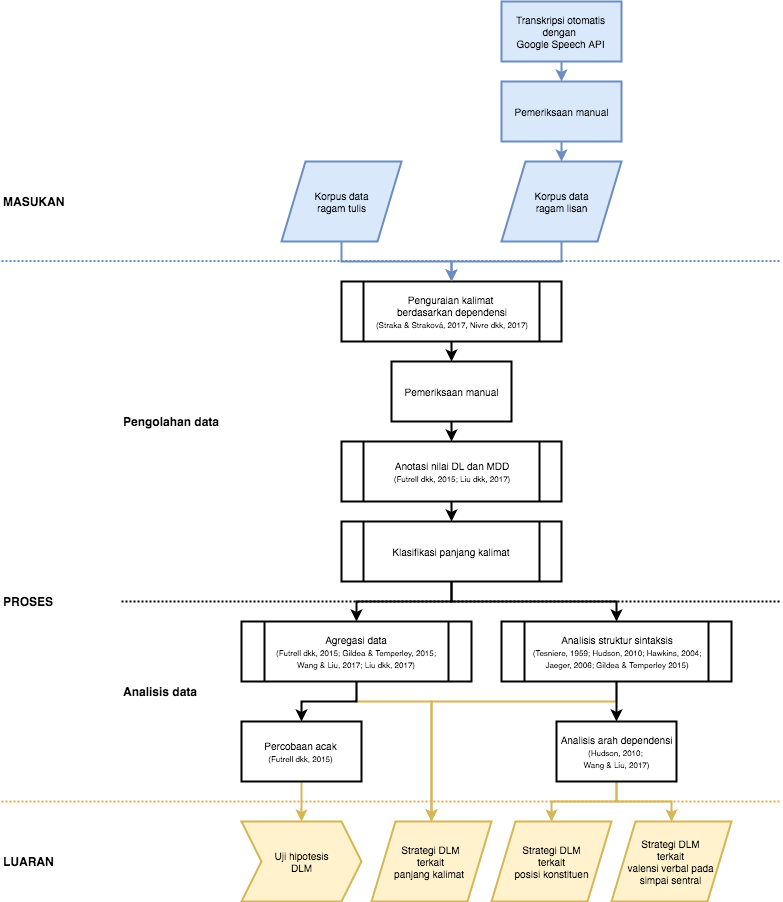
\includegraphics[width=1
	\textwidth] {pics/kerangka-konseptual.png} \caption{Diagram alur kerangka konseptual penelitian} 
\label{fig:kerangka-konseptual} \end{figure}

%-----------------------------------------------------------------------------%

